\documentclass[aspectratio=169,11pt]{beamer}
% ==========================================================================
%  KSA lecture-slide theme  =  stock beamer "Boadilla"  +  KSA colour theme
%  brand colours sampled from the official KSA symbol mark:
%    Deep Prussian Blue  #2E3192   (지성 - intellect)
%    Golden Gray         #D6CBB1   (감성 - sensibility)
%  Engine: XeLaTeX.  Usage:
%    \documentclass[aspectratio=169,11pt]{beamer}
%    \input{../../theme/ksa-theme.tex}
%  Each deck lives in its own slides/kor/<deck>/ folder together with its
%  own images; ../../figs/ is kept only as a fallback for the shared cache.
% ==========================================================================

\usepackage{fontspec}
\usepackage{amsmath,amssymb}
\usepackage{graphicx}
\graphicspath{{figs/}{./}{../../../figs/}}
\usepackage{booktabs}
\usepackage{listings}
\usepackage{varwidth}

% ---- fonts (no ctex/xeCJK on this box -> fontspec drives CJK directly) -----
\defaultfontfeatures{Ligatures=TeX}
\setmainfont{Noto Sans CJK KR}
\setsansfont{Noto Sans CJK KR}
\setmonofont{Noto Sans Mono CJK KR}[Scale=0.92]

% ---- base theme: stock Boadilla ------------------------------------------
\usetheme{Boadilla}
\usefonttheme{professionalfonts}
\setbeamertemplate{navigation symbols}{}

% ---- KSA colour theme (recolour the stock theme) --------------------------
\definecolor{ksablue}{HTML}{2E3192}
\definecolor{ksabluedk}{HTML}{20226A}
\definecolor{ksagold}{HTML}{D6CBB1}
\definecolor{ksagolddk}{HTML}{A9976B}
\definecolor{ksared}{HTML}{C0392B}
\definecolor{ksagray}{HTML}{5B5B5B}

\setbeamercolor{structure}{fg=ksablue}
\setbeamercolor{alerted text}{fg=ksared}

\setbeamercolor{palette primary}{fg=white,           bg=ksablue}
\setbeamercolor{palette secondary}{fg=white,         bg=ksablue!85!black}
\setbeamercolor{palette tertiary}{fg=white,          bg=ksabluedk}
\setbeamercolor{titlelike}{fg=ksablue}
\setbeamercolor{frametitle}{fg=ksablue,bg=}
\setbeamercolor{title}{fg=ksablue}
\setbeamercolor{author}{fg=ksagray}
\setbeamercolor{institute}{fg=ksagray}
\setbeamercolor{block title}{fg=white,bg=ksablue}
\setbeamercolor{block body}{fg=black!85,bg=ksablue!6}
\setbeamercolor{item}{fg=ksablue}
\setbeamercolor{section in toc}{fg=black!85}

\setbeamerfont{frametitle}{series=\bfseries}
\setbeamerfont{title}{series=\bfseries}

% ---- footline:  KSA mark | "Made by ..." | n / N   (matches reference) ----
\newcommand{\ksacredit}{}
\setbeamertemplate{footline}{%
  \hbox{%
    \begin{beamercolorbox}[wd=.18\paperwidth,ht=2.6ex,dp=1.5ex,leftskip=1.1em]{}%
      \raisebox{-0.35ex}{\includegraphics[height=2.0ex]{ksa-logo.png}}%
    \end{beamercolorbox}%
    \begin{beamercolorbox}[wd=.64\paperwidth,ht=2.6ex,dp=1.5ex,center]{}%
      {\scriptsize\color{ksagray}\ksacredit}%
    \end{beamercolorbox}%
    \begin{beamercolorbox}[wd=.18\paperwidth,ht=2.6ex,dp=1.5ex,rightskip=1.1em]{}%
      \hfill{\scriptsize\color{ksablue}\insertframenumber\,/\,\inserttotalframenumber}%
    \end{beamercolorbox}%
  }%
  \vskip2pt
}

% ---- section divider: stock \sectionpage, KSA-coloured -------------------
\setbeamertemplate{section page}{%
  \begingroup\centering
    {\color{ksagolddk}\rule{0.16\paperwidth}{1pt}}\par\vskip1.0em
    {\usebeamerfont{title}\color{ksablue}\insertsectionhead\par}\vskip1.0em
    {\color{ksagolddk}\rule{0.16\paperwidth}{1pt}}\par
  \endgroup
}
\AtBeginSection[]{\begin{frame}[plain,noframenumbering]\vfill\sectionpage\vfill\end{frame}}

% ---- code listings ------------------------------------------------------------
\lstdefinestyle{ksa}{%
  basicstyle=\ttfamily\scriptsize,
  keywordstyle=\color{ksablue}\bfseries,
  commentstyle=\color{ksagray}\itshape,
  stringstyle=\color{ksagolddk},
  numberstyle=\tiny\color{ksagray},
  backgroundcolor=\color{ksablue!6},
  frame=leftline, framerule=1.4pt, rulecolor=\color{ksablue},
  xleftmargin=1em, aboveskip=0.8em, belowskip=0.4em,
  showstringspaces=false, breaklines=true, language=Python,
}
\lstset{style=ksa}

% ---- handy macros -----------------------------------------------------------
\newcommand{\kb}[1]{\textbf{\color{ksablue}#1}}   % blue keyword
\newcommand{\kq}[1]{\textbf{\color{ksared}#1}}    % red key-question

\setbeamerfont{title}{series=\bfseries,size=\fontsize{24}{30}\selectfont}
\setbeamerfont{subtitle}{series=\bfseries,size=\fontsize{14}{18}\selectfont}
\setbeamerfont{author}{size=\normalsize}
\setbeamerfont{institute}{size=\small}
\graphicspath{{figs/}{../../../../assets/}}
\makeatletter
\newcommand{\markpage}[1]{\protected@write\@auxout{}{\string\newlabel{#1}{{\the\c@framenumber}{}}}\hypertarget{#1}{}}
\newcommand{\pref}[1]{\hyperlink{#1}{\textcolor{ksagolddk}{(p.\ref{#1})}}}
\makeatother

\renewcommand{\ksacredit}{Machine Learning 1 \,\textperiodcentered\, 트랜스포머}
\title{트랜스포머 (Transformer)}
\subtitle{모든 단어를 한 번에 보는 블록을 쌓는다}
\author{Machine Learning 1}
\institute{한국과학영재학교 (KSA)}
\date{}
\begin{document}
\begin{frame}[plain,noframenumbering]\titlepage\end{frame}


% --- 오늘의 질문
\begin{frame}{오늘의 질문: ChatGPT 의 T 는?}
\vfill
\centering
{\LARGE Chat \quad \textcolor{ksagray}{G}enerative \quad \textcolor{ksagray}{P}re-trained \quad \kb{T}ransformer}\vskip1.2em
{\large 2017년 구글 논문 ``\textbf{Attention Is All You Need}'' (Vaswani 외 8명)}\\[0.5em]
{\large 지금의 언어 모델 · 번역기 · 이미지 생성기 대부분이 이 구조 위에 있다}
\vfill
\note{ChatGPT의 G, P, T에서 마지막 T는 무엇의 약자일까요? 트랜스포머입니다. G는 글을 만들어 낸다는 뜻의 Generative, P는 미리 학습했다는 Pre-trained입니다. 트랜스포머는 2017년 구글 연구자들의 논문 Attention Is All You Need에서 나왔습니다. 지금의 언어 모델, 번역기, 이미지 생성기 대부분이 이 구조 위에 있습니다. 지난 시간에 배운 어텐션만으로 어떻게 이런 모델을 만드는지 봅시다.}
\end{frame}

% --- RNN vs 트랜스포머
\begin{frame}{RNN 은 차례로, 트랜스포머는 한 번에}
\markpage{seq}
\vfill
\centering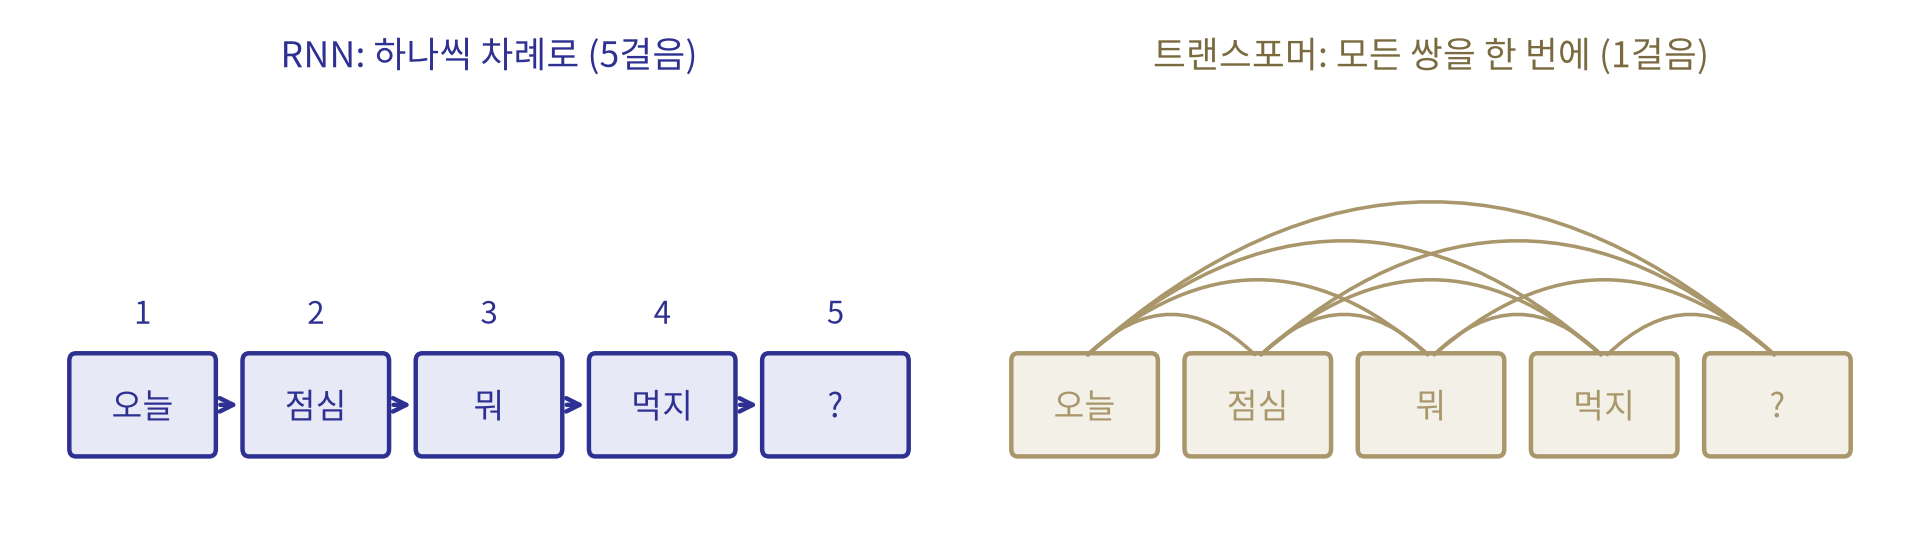
\includegraphics[width=0.9\linewidth]{tf_seq.png}\par\vskip0.3em
\renewcommand{\arraystretch}{1.3}
{\large\begin{tabular}{lcc}
 & RNN & 트랜스포머 (셀프 어텐션)\\\hline
단어 $n$ 개를 읽는 차례 & $n$ 걸음 (앞이 끝나야 뒤) & \kb{1} 걸음 (모두 동시에, GPU)\\
첫 단어 $\leftrightarrow$ 끝 단어 & $n - 1$ 걸음 거쳐 전달 & \kb{바로} 연결\\
계산량 & $n$ 에 비례 & 모든 쌍: $n^2$ 에 비례
\end{tabular}}
\vfill
\note{RNN은 단어를 하나씩 차례로 읽습니다. 앞 단어를 다 계산해야 다음 단어로 갈 수 있으니, 다섯 단어면 다섯 걸음입니다. 첫 단어의 정보가 끝 단어에 가려면 중간 칸을 모두 거쳐야 해서, LSTM을 써도 멀면 흐려집니다. 트랜스포머는 셀프 어텐션으로 모든 단어 쌍을 한 번에 봅니다. 순서를 기다릴 필요가 없으니 GPU로 모든 칸을 동시에 계산하고, 첫 단어와 끝 단어도 바로 연결됩니다. 대신 모든 쌍을 보니 계산량이 단어 수의 제곱에 비례합니다. 긴 글이 비싼 이유입니다.}
\end{frame}

% --- 셀프 어텐션 + 멀티헤드
\begin{frame}{셀프 어텐션, 여러 개의 머리로}
\vfill
\centering
{\large 단어 벡터 $X$ ($n$ × 512) 에서 \quad $Q = X W_Q, \ K = X W_K, \ V = X W_V$}\\[0.3em]
{\Large\[ \text{head} = \text{softmax}\!\left(\frac{Q K^\top}{\sqrt{64}}\right) V \]}\vskip0.2em
\renewcommand{\arraystretch}{1.4}
{\large\begin{tabular}{ll}
\textbf{멀티헤드} & 512칸을 \kb{8개 머리} × 64칸으로 나눠 따로 $\to$ 이어 붙여 $W_O$\\
왜 여러 개? & 머리마다 다른 관계 (주어 $\leftrightarrow$ 동사, ``그것은'' $\leftrightarrow$ 동물)
\end{tabular}}\\[0.6em]
{\small 지난 시간과 달리 $Q, K, V$ 를 \textbf{학습하는 행렬}로: 무엇을 찾을지 · 내걸지 · 줄지를 배운다}
\vfill
\note{트랜스포머의 셀프 어텐션은 지난 시간 그것은 예제와 같지만 한 가지가 다릅니다. 쿼리, 키, 밸류를 단어 벡터 그대로 쓰지 않고, 각각 학습하는 행렬 W_Q, W_K, W_V를 곱해 만듭니다. 그래서 무엇을 찾을지, 무엇을 내걸지, 무엇을 줄지를 배웁니다. 또 원 논문은 512칸을 64칸씩 8개로 나눠 어텐션을 8번 따로 합니다. 이걸 멀티헤드라고 합니다. 머리마다 주어와 동사, 대명사와 가리키는 말처럼 서로 다른 관계를 볼 수 있습니다. 8개 결과를 이어 붙여 행렬 W_O를 곱하면 다시 512칸이 됩니다.}
\end{frame}

% --- 위치 정보
\begin{frame}{순서는? 위치 정보를 더한다}
\markpage{pe}
\vfill
\centering
{\large 셀프 어텐션은 순서를 모른다: Dog bites man = Man bites dog (\textbf{같은 쌍}들)}\vskip0.3em
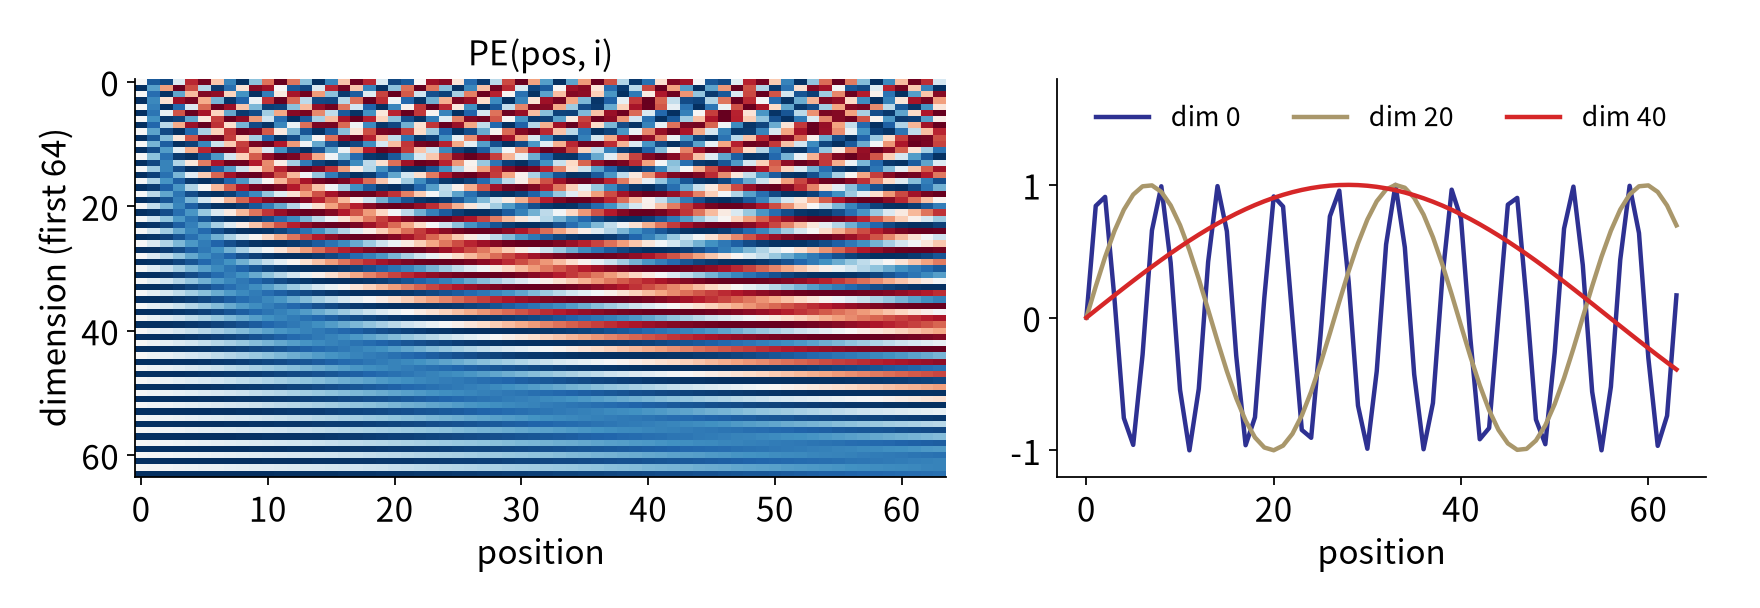
\includegraphics[width=0.72\linewidth]{tf_pe.png}\par
{\large 입력 = 단어 벡터 + \kb{위치 벡터} \quad $\text{PE}(pos, 2i) = \sin\!\left(pos / 10000^{2i/d}\right)$, \quad $2i + 1$ 칸은 $\cos$}\\[0.2em]
{\small 칸마다 주기가 다른 물결 $\to$ 위치마다 다른 무늬 \quad 위치 벡터를 학습으로 정해도 비슷하다 (논문, GPT)}
\vfill
\note{모든 단어를 한 번에 보면 문제가 하나 생깁니다. 셀프 어텐션은 단어 쌍의 비슷함만 보니까 순서를 모릅니다. 11주차에 본 Dog bites man과 Man bites dog을 구분하지 못합니다. 그래서 단어 벡터에 위치를 나타내는 벡터를 더합니다. 원 논문은 사인과 코사인을 썼습니다. 칸마다 주기가 다른 물결이라, 왼쪽 그림처럼 위치마다 다른 무늬가 생깁니다. 앞 칸은 빨리, 뒤 칸은 천천히 바뀝니다. 시계의 초침, 분침, 시침처럼요. 위치 벡터를 학습으로 정해도 결과가 비슷하다고 논문에 나오고, GPT는 학습하는 방식을 씁니다.}
\end{frame}

% --- 블록
\begin{frame}{블록 하나: 주고받고, 다듬고}
\markpage{block}
\vfill
\begin{columns}[c]
\column{0.38\linewidth}\centering
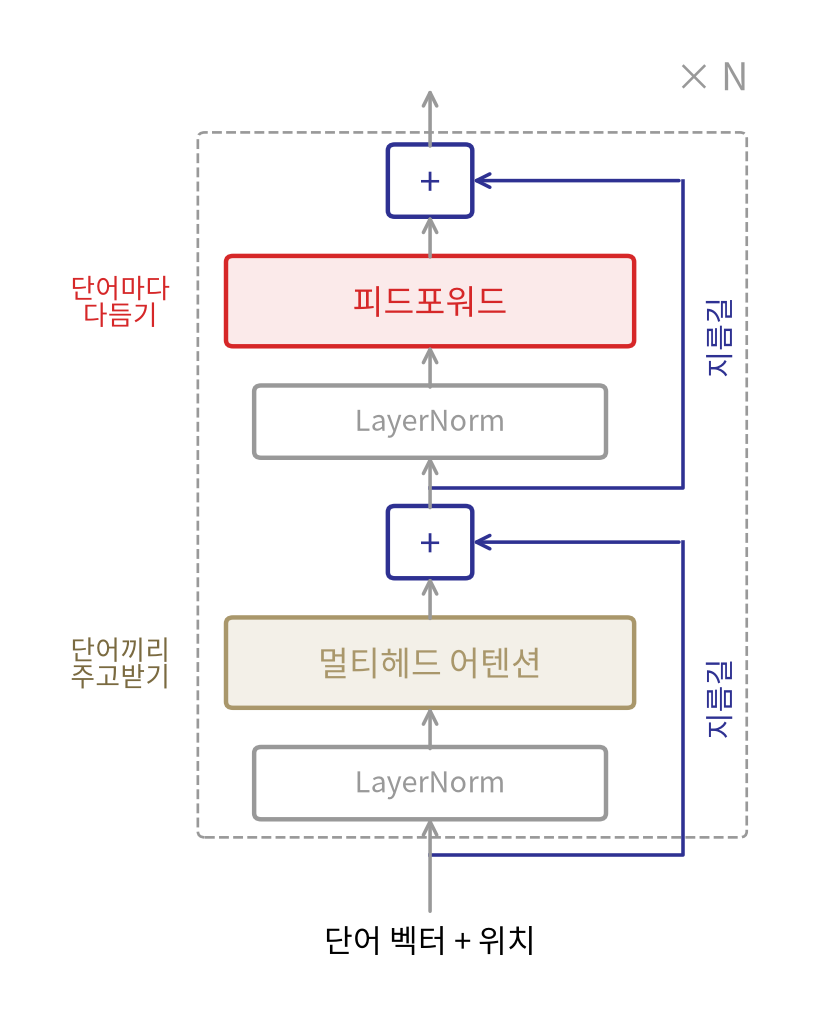
\includegraphics[width=\linewidth]{tf_block.png}
\column{0.6\linewidth}
\renewcommand{\arraystretch}{1.5}
{\large\begin{tabular}{ll}
\textcolor{ksagolddk}{어텐션} & 단어끼리 정보를 \textbf{주고받는다}\\
\textcolor{ksared}{피드포워드} & 단어마다 따로 \textbf{다듬는다}\\
 & 512 $\to$ 2048 $\to$ 512 (ReLU)\\
\textcolor{ksablue}{지름길} & $x + f(x)$: ResNet (10주차)\\
LayerNorm & 단어마다 평균 0 · 분산 1 로
\end{tabular}}\\[0.6em]
{\large 이 블록을 \kb{N 번} 쌓는다}\\[0.2em]
{\small 그림은 GPT 등이 쓰는 순서 (정규화 먼저) \quad 원 논문은 더한 뒤 정규화}
\end{columns}
\vfill
\note{트랜스포머 블록 하나는 두 단계입니다. 먼저 멀티헤드 어텐션으로 단어끼리 정보를 주고받고, 다음으로 피드포워드 신경망으로 단어마다 따로 다듬습니다. 피드포워드는 512칸을 2048칸으로 넓혔다가 다시 512칸으로 줄이는 2층 신경망입니다. 각 단계에는 ResNet에서 배운 지름길이 붙어서, 입력에 결과를 더합니다. 그래서 깊게 쌓아도 학습이 됩니다. LayerNorm은 단어마다 벡터를 평균 0, 분산 1로 맞춥니다. 9주차 배치 정규화와 비슷하지만 단어 하나 안에서 합니다. 이 블록을 N번 쌓으면 트랜스포머입니다.}
\end{frame}

% --- 가중치 세기
\begin{frame}{손으로 세기: 블록 하나의 가중치}
\markpage{count}
\vfill
\centering
\renewcommand{\arraystretch}{1.5}
{\large\begin{tabular}{lll}
어텐션 & $W_Q, W_K, W_V, W_O$: \quad $d \times d$ 네 개 & $4d^2$\\
피드포워드 & $d \times 4d$, \quad $4d \times d$ & $8d^2$\\\hline
블록 하나 & & \kb{$12 d^2$} \quad (편향 · 정규화 빼고)
\end{tabular}}\vskip0.8em
\renewcommand{\arraystretch}{1.4}
{\large\begin{tabular}{lccr}
 & $d$ & 층 & 가중치 $\approx 12 d^2 \times$ 층\\\hline
원 논문 (인코더 6층) & 512 & 6 & $3.1\text{M} \times 6 \approx 19\text{M}$\\
GPT-3 (2020) & 12,288 & 96 & $1.8\text{B} \times 96 \approx$ \kb{174B}
\end{tabular}}\\[0.5em]
{\large GPT-3 의 1,750억 개가 거의 이 식 하나로 나온다}
\vfill
\note{블록 하나에 가중치가 몇 개인지 세 봅시다. 어텐션에는 d 곱하기 d 행렬이 Q, K, V, 출력용으로 4개, 4 d 제곱입니다. 멀티헤드로 나눠도 합치면 같습니다. 피드포워드는 d에서 4d로, 4d에서 d로 가는 행렬 두 개라 8 d 제곱입니다. 합치면 블록 하나에 12 d 제곱입니다. 원 논문은 d가 512이니 블록 하나에 약 310만 개, 인코더 6층이면 약 1900만 개입니다. GPT-3은 d가 12288, 96층이라 12 곱하기 12288 제곱 곱하기 96, 약 1740억 개입니다. 발표된 1750억 개가 거의 이 식 하나로 나옵니다.}
\end{frame}

% --- 앞만 보기
\begin{frame}{GPT: 앞 단어만 보고 다음 단어 맞히기}
\vfill
\begin{columns}[c]
\column{0.4\linewidth}\centering
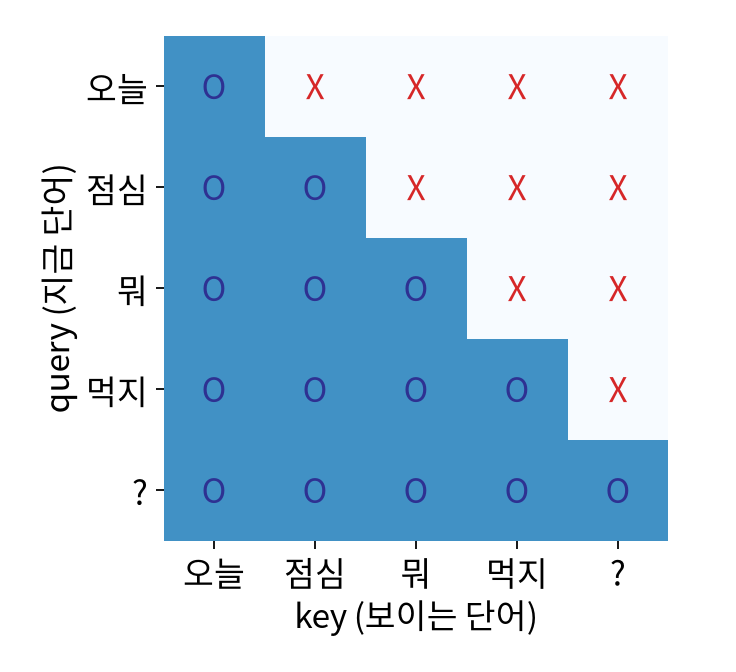
\includegraphics[width=\linewidth]{tf_mask.png}
\column{0.58\linewidth}
{\large 다음 단어를 맞히는데 뒤 단어를 보면 반칙}\\[0.3em]
{\large $\to$ 점수 행렬의 위쪽을 $-\infty$ 로 (softmax 후 0)}\\[0.8em]
\renewcommand{\arraystretch}{1.4}
{\large\begin{tabular}{ll}
원 논문 & 인코더 6층 + 디코더 6층 (번역)\\
BERT (2018) & 인코더만: 양쪽 다 본다\\
GPT (2018 $\sim$) & 디코더만: \kb{앞만} 본다
\end{tabular}}\\[0.5em]
{\small 칸 하나의 앞만 보기로 길이 $n$ 문장에서 $n$ 개 문제를 한 번에 학습}
\end{columns}
\vfill
\note{GPT는 앞 단어들을 보고 다음 단어를 맞히도록 학습합니다. 그런데 셀프 어텐션은 모든 단어를 한 번에 보니까, 그대로 두면 뒤 단어, 즉 정답을 봐 버립니다. 그래서 점수 행렬의 위쪽 절반을 마이너스 무한대로 바꿔 softmax 뒤 0이 되게 합니다. 그림처럼 먹지는 오늘, 점심, 뭐, 먹지까지만 봅니다. 원 논문은 번역을 위해 인코더 6층과 디코더 6층을 썼고, BERT는 인코더만 써서 양쪽을 다 보고, GPT는 디코더만 써서 앞만 봅니다. 앞만 보게 하면 길이 n 문장 하나로 다음 단어 문제 n개를 한 번에 학습할 수 있습니다.}
\end{frame}

% --- 논문 결과
\begin{frame}{논문 결과 (2017)}
\vfill
\centering
\renewcommand{\arraystretch}{1.5}
{\large\begin{tabular}{lll}
영어 $\to$ 독일어 (WMT'14) & BLEU \kb{28.4} & 기존 최고 +2 점 넘게\\
영어 $\to$ 프랑스어 & BLEU \kb{41.8} & GPU 8개로 3.5일 (훨씬 적은 계산)\\
base 모델 & & GPU 8개로 \textbf{12시간}
\end{tabular}}\vskip0.8em
{\large RNN 없이 어텐션만으로 더 잘, 더 빨리 \quad $\to$ 제목: Attention Is All You Need}
\vfill
\note{2017년 논문의 결과입니다. 영어 독일어 번역에서 BLEU 28.4점으로 앙상블을 포함한 기존 최고 기록보다 2점 넘게 높았고, 영어 프랑스어 번역에서는 41.8점을 GPU 8개로 3.5일 학습해 얻었습니다. 기존 모델들의 학습 비용보다 훨씬 적은 계산입니다. 작은 base 모델은 GPU 8개로 12시간이면 충분했습니다. RNN 없이 어텐션만으로 더 잘, 더 빨리 학습했다, 그래서 제목이 어텐션만 있으면 된다입니다.}
\end{frame}

% --- 실험
\begin{frame}{실험: 셰익스피어 글자 모델, 트랜스포머로}
\markpage{exp}
\vfill
\begin{columns}[c]
\column{0.55\linewidth}\centering
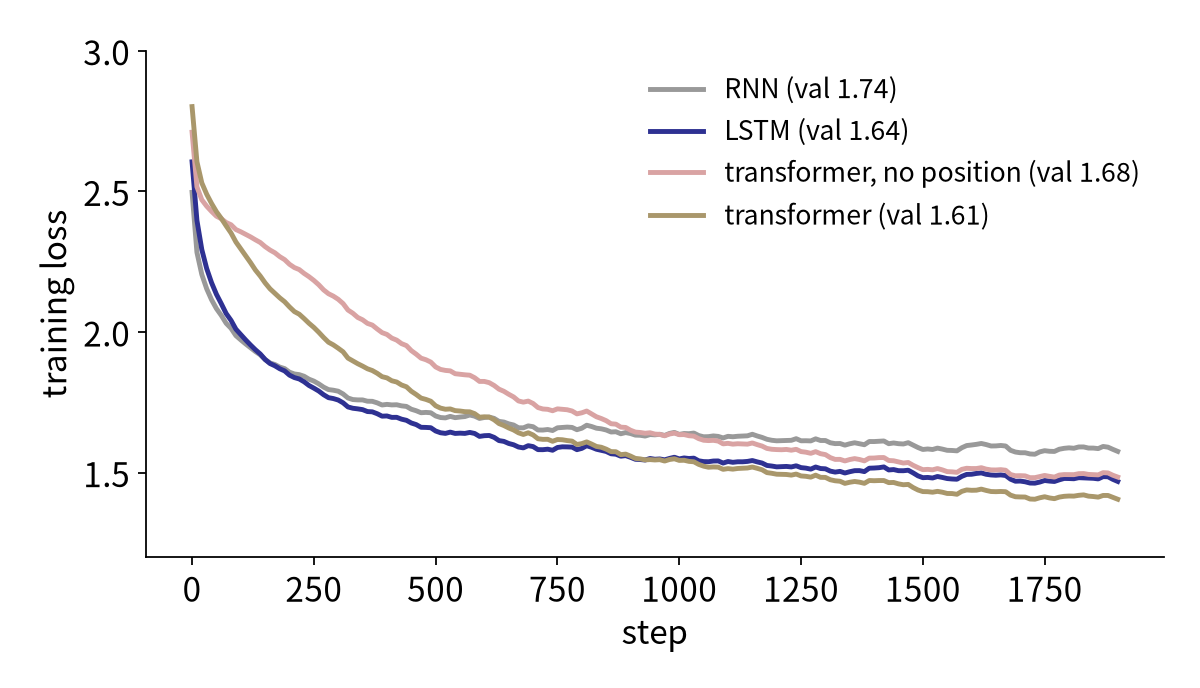
\includegraphics[width=\linewidth]{tf_curve.png}
\column{0.43\linewidth}\centering
\renewcommand{\arraystretch}{1.3}
{\normalsize\begin{tabular}{lcr}
 & 검증 손실 & 가중치\\\hline
RNN & 1.74 & 5만\\
LSTM & 1.64 & 15만\\
트랜스포머 & \kb{1.61} & 82만\\
\quad 위치 정보 뺌 & 1.68 & 82만
\end{tabular}}\\[0.6em]
{\small 폭 128 · 4층 · 머리 4 \quad 11주차와 같은 조건 (조각 64, 2,000걸음)}\\[0.3em]
{\small 이 작은 CPU 실험에서는 한 걸음이 LSTM 의 약 3배 느렸다: 장점은 GPU · 긴 글 · 큰 모델에서 나온다}
\end{columns}
\vfill
\note{11주차 셰익스피어 글자 모델을 같은 조건으로 트랜스포머로 학습했습니다. 폭 128, 4층, 머리 4개의 작은 GPT입니다. 검증 손실은 RNN 1.74, LSTM 1.64, 트랜스포머 1.61로 가장 낮습니다. 다만 가중치가 82만 개로 더 많으니 공정한 비교는 아닙니다. 위치 정보를 빼면 1.68로 나빠집니다. 순서를 모르면 손해라는 뜻이죠. 앞만 보기 때문에 몇 번째 단어인지 어렴풋이 알 수 있어서 완전히 망가지지는 않습니다. 그리고 솔직히 말하면, 이 작은 CPU 실험에서는 트랜스포머 한 걸음이 LSTM보다 약 3배 느렸습니다. 트랜스포머의 속도 장점은 GPU로 긴 글과 큰 모델을 학습할 때 나옵니다.}
\end{frame}

% --- 쌓기
\begin{frame}{블록을 쌓아 온 길}
\vfill
\centering
\renewcommand{\arraystretch}{1.5}
{\large\begin{tabular}{llll}
2017 & 원 논문 & 인코더 6층 + 디코더 6층 & 번역\\
2018 & BERT & 인코더 24층 (large) & 문장 이해 (14주차)\\
2020 & GPT-3 & 디코더 \kb{96층}, 1,750억 개 & 글 쓰기\\
2020 & ViT & 이미지 조각을 단어처럼 & 이미지 분류
\end{tabular}}\vskip0.8em
{\large 블록은 거의 그대로, \textbf{층 · 폭 · 데이터}를 키웠다}
\vfill
\note{트랜스포머 블록은 2017년 이후 거의 그대로 쓰이고, 층과 폭과 데이터를 키워 왔습니다. 2018년 BERT는 인코더만 24층 쌓아 문장 이해에 썼고, 14주차에 배웁니다. 2020년 GPT-3은 디코더만 96층, 1750억 개로 글을 씁니다. 같은 해 ViT는 이미지를 작은 조각으로 잘라 단어처럼 넣어 이미지 분류도 트랜스포머로 했습니다.}
\end{frame}

% --- 문제풀이
\begin{frame}{문제풀이}
\vfill
\begin{enumerate}
\item $d = 768$, 12층 (GPT-2 small, BERT base) 의 블록 가중치는 대략 몇 개? ($12 d^2 \times$ 층)\vskip0.8em
\item 단어 1,000개 문장에서 셀프 어텐션 점수는 몇 개 계산하나? 10,000개면 몇 배?\vskip0.8em
\item 앞만 보기 마스크에서 단어 5개 문장의 0 이 아닌 칸은 몇 개인가?\vskip0.8em
\item 위치 정보를 빼도 앞만 보는 모델은 손실 1.68 로 꽤 배웠다. 어떻게 위치를 짐작할 수 있었을까?
\end{enumerate}
\vfill
\note{1번 답. 12 곱하기 768 제곱 곱하기 12, 약 8500만 개입니다. 단어 벡터까지 더하면 약 1억 1천만 개, 발표된 크기와 비슷합니다. 2번 답. 1000 제곱, 100만 개이고, 10000개면 1억 개로 100배입니다. 길이가 10배면 계산은 100배입니다. 3번 답. 1 더하기 2 더하기 3 더하기 4 더하기 5, 15칸입니다. 4번 답. 첫 단어는 자기 하나만, 열 번째 단어는 열 개를 봅니다. 보는 단어 수가 달라 어텐션 결과가 위치마다 달라지니, 위치를 어렴풋이 알 수 있습니다.}
\end{frame}

% --- 실습
\begin{frame}{실습}
\vfill
\centering\begin{tabular}{rl}
\large 1 & 위치 정보 만들기 (사인 · 코사인), 앞만 보기 마스크\\[0.5em]
\large 2 & 트랜스포머 블록 직접 쌓기 $\to$ 가중치 수를 $12 d^2$ 와 비교\\[0.5em]
\large 3 & 셰익스피어 작은 GPT 학습 $\to$ 글 써 보기
\end{tabular}\vskip1em
Tiny Shakespeare (Karpathy, char-rnn) \\[0.4em]\href{https://colab.research.google.com/github/SuminHan/book-ml/blob/main/slides/v2/ml1/week12/transformer/lab/transformer.ipynb}{\textcolor{ksagolddk}{▶ Colab에서 실습 노트북 열기}}
\vfill
\note{실습은 세 부분입니다. 첫째, 사인과 코사인으로 위치 정보를 만들고 앞만 보기 마스크를 만듭니다. 둘째, PyTorch로 트랜스포머 블록을 직접 쌓고 가중치 수를 12 d 제곱 식과 비교합니다. 셋째, 셰익스피어 글자 데이터로 작은 GPT를 학습해 글을 써 봅니다.}
\end{frame}

% --- 정리
\begin{frame}{정리}
\vfill
\centering\large\begin{tabular}{l}
\textbf{트랜스포머}: RNN 없이 셀프 어텐션으로 모든 단어를 \kb{한 번에} (2017)\\[0.5em]
입력 = 단어 + 위치 \quad 블록 = 멀티헤드 어텐션 $\to$ 피드포워드, 지름길 · LayerNorm\\[0.5em]
블록 하나 $\approx 12 d^2$ \quad GPT-3: $12 \times 12288^2 \times 96 \approx 1{,}750$억\\[0.5em]
GPT = 앞만 보는 디코더 \quad 셰익스피어 검증 손실 1.64 (LSTM) $\to$ 1.61
\end{tabular}
\vfill
\note{정리합니다. 트랜스포머는 RNN 없이 셀프 어텐션으로 모든 단어를 한 번에 봅니다. 순서를 모르니 단어 벡터에 위치 벡터를 더하고, 블록 하나는 멀티헤드 어텐션으로 주고받고 피드포워드로 다듬으며, 지름길과 LayerNorm이 붙습니다. 블록 하나의 가중치는 약 12 d 제곱이고, GPT-3의 1750억 개가 이 식으로 나옵니다. GPT는 앞만 보는 디코더이고, 셰익스피어 실험에서는 LSTM의 1.64보다 낮은 1.61을 얻었습니다.}
\end{frame}
\end{document}
